\documentclass[a4paper, 11pt]{article}
\usepackage[T1]{fontenc}
\usepackage{subfigure}
\usepackage[margin=2.5cm, nohead]{geometry}
\usepackage{palatino, url, multicol}
\usepackage{amssymb, graphicx, fancyhdr, latexsym, url, verbatim}
\usepackage{algorithm, algorithmic}
\usepackage{hyperref}
\usepackage{clrscode3e}
\usepackage[all]{xy}
\usepackage[english]{babel}
\usepackage{matlabScripts}
\usepackage{caption}


\newcommand{\projectName}{ACHTBITS}
\newcommand{\projectAbbreviation}{Awesome
CHaradriiformes Toegepast BIrd Tracking System}
\newcommand{\bits}{BITS}

\addtolength{\footskip}{-90mm}
\addtolength{\headheight}{-05mm}
\addtolength{\headsep}{05mm}

%\pagestyle{fancy}
\lhead{\projectName}
%\chead{Annotation Tool - User Guide}
\rhead{\small \textsc{\projectAbbreviation}}
%\cfoot{\footnotesize \textit{ \projectAbbreviation}\\[0.1cm] \small \thepage}
%\cfoot{}
%\rfoot{\thepage}


\setlength{\parindent}{0pt}
\setlength{\parskip}{10pt}

\begin{document}

\newcommand{\HRule}{\rule{\linewidth}{0.5mm}}

\begin{titlepage}
\begin{center}

\includegraphics[width=1\textwidth]{uva}\\[0.5cm]

\HRule \\[0.2cm]
{ \huge \LARGE \textbf{\projectName}\\[0.1cm]
\large \textsc{\projectAbbreviation}
 \vspace{0.2cm}}
\HRule \\[0.4cm]
\Large \today

\vfill

\begin{tabular}{cccc}
Jesse Eisses & Sosha Happel & Maarten Inja & Maarten de Waard \\ 
6352189 & 6273831 & 5872464 & 5894883 
\end{tabular} \\[0.3cm]

\large \{mrtndwrd, maarten.inja, jesse.eisses, soshappel\}@gmail.com 
\end{center}
\end{titlepage}

%%{
%\begin{center}
%% Upper part of the page
%
%\textmd{Leren en Beslissen verslag}
%\vfill
%% Title
%{ \huge \textbf{ACHTBITS} \\\large \textsc{Awesome Charadriiformes Toegepast
%BIrd Tracking System}
%}\\[0.4cm]
%%\begin{center}
%\vfill
%By\\
%\vfill
%%\large\textbf{{Maarten de Waard \\ 5894883},  {Maarten Inja \\ 5872464},  {Jesse Eisses \\
%%6352189}, {Sosha Happel \\ 6273831}}
%\begin{tabular}{cccc}
%Jesse Eisses & Sosha Happel & Maarten Inja & Maarten de Waard \\ 
%6352189 & 6273831 & 5872464 & 5894883 
%\end{tabular}
%\vfill
%\{mrtndwrd, maarten.inja, jesse.eisses, soshappel\}@gmail.com
%%6352189 \and Sosha Happel\\ 6273831}
%\end{center}
%
%\end{titlepage}
%%}

%\thispagestyle{empty}
\vspace*{00mm}
\tableofcontents
\newpage

\section{Overview}
% Overview of the functionality of the tool

This tool was created to aid the annotation of data from the UvA-BITS (BIrd Tracking System) database, in particular data of the lesser black-backed gull above the North sea. The tool contains:
\begin{itemize}
\item
a script that reads raw data downloaded from the database and creates flight-sessions.
\item
an automated segmentation algorithm that splits sessions into clusters that are likely to belong to the same class of behaviours 
\item
a GUI that shows information about a cluster and lets the user choose a behaviour class.
\item
A shell that runs through all sessions of a device and calls the annotation tool
\item
Functions to prepare the annotated data for a classification algorithm
\end{itemize}

\section{Installation}
% short explanation of how to get the tool ready for use

\section{Usage}
\subsection{Preparing Data}
% how to get data from the database ready for the tool
 
\subsection{Annotating Sessions and Clusters}

The main function to use the annotation tool is annotateBird, this functions takes a deviceId loops through all sessions in the folder of the device and puts them into the tool. The classes given as user input are added to the features of the cluster and saves them to a file.\\ \\

Layout:
\begin{enumerate}
	\item button control
	\begin{enumerate}
		\item
		exit - closes the tool\\
		back - returns to the previous cluster
		\item
		zoom in - zooms in on the whole session\\
		zoom out - zooms out to the entire coast of the Netherlands
		\item
		classes - a group of class buttons used to annotate the current cluster
	\end{enumerate}
	\item
	plot of the trajectory of the session\\
	the current cluster is highlighted in light blue\\
	the start of the session is marked with a red square\\
	the start of the current cluster is marked by a green square\\
	the previous clusters are color coded with their class
	\item
	plot of the trajectory of the current cluster\\
	the start of the cluster is marked by a green square
	\item
	accelerometer-data plots of the points marked by a vertical line in the velocity plot
	\item
	velocity and acceleration plot
	\item
	instantaneous speed and direction vectors
	\item
	features of the current cluster
	
\end{enumerate}
		
 % running and using the tool
\begin{figure}[h]
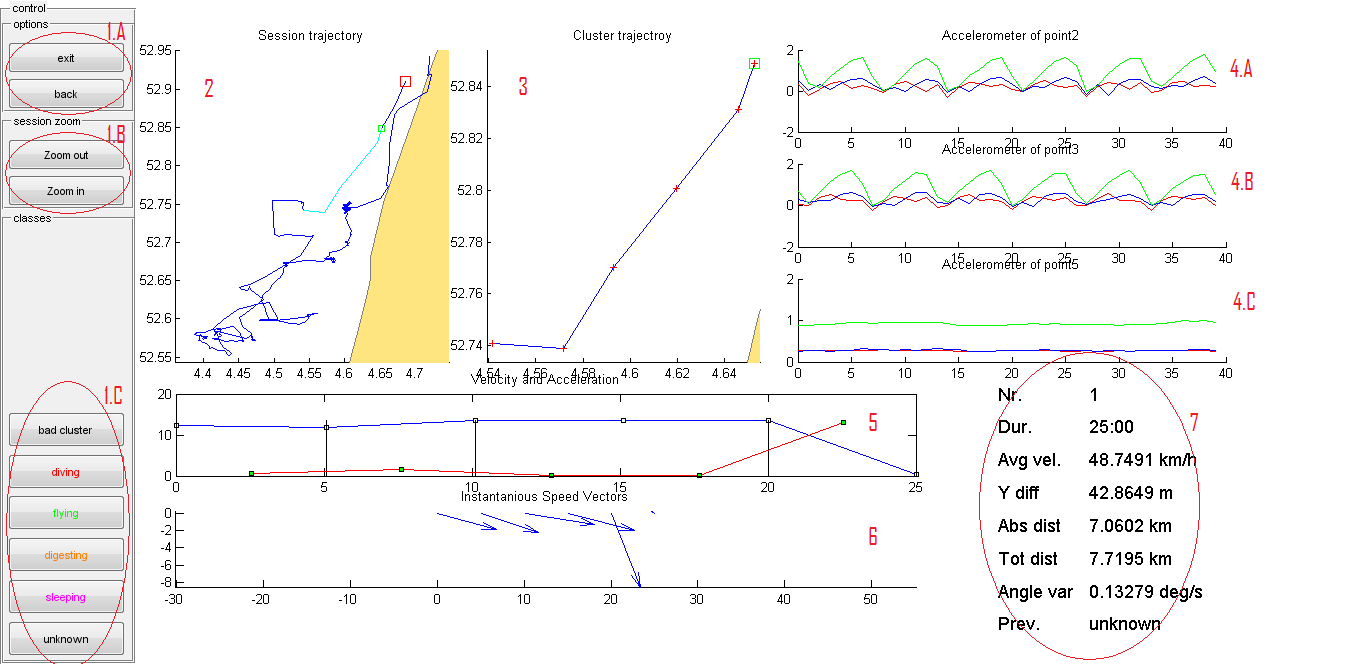
\includegraphics[scale = 0.5]{tool_overview_indexed.png}
\end{figure}
\subsection{Using the Resulting Annotated Features}
% what the tool outputs and how this can be adjusted

\section{Making Adjustments}
% things that could be added and how this should be done

\subsection{Adjusting Parameters}

\subsection{Explanation of main functions}

\end{document}
